% !TeX root = ./main.tex

\section{Methodology}
By far the largest part of this work was the surveying and preprocessing of the data to transform it into a conforming format. "Conforming" means here that the result is usable by the different frameworks used for training. For this the the data files needed to be altered in such a way that per student only one row remained. These rows then can be appended to each study spell of the student, forming a coherent dataframe where each row represents one input vector plus the target value. The data is fed as an input vector, and several rows, containing information on the same variable is not simply convertible into one single vector, since one variable can only contain one value. The most simple appraoch would be to append all rows together, but since there are different amount of rows per student, all others would need to be padded to the maximum length, resulting in a larger amount of additional NaN values. Hence, another appraoch needed to be taken to aggregate the several rows. The preprocessed data could then be fed into the different machine learning algorithms used. The algorithms can be tuned with different hyperparameters slightly changing their behaviour. They learn the most important features to predict the outcome. For some of the models the learning can then be evaluated.\\
The data processing was handled with pandas (v0.24.2)\cite{WesMcKinney.2010} and numpy (v1.16.2)\cite{vanderWalt.2011}. The training and evaluation was done in scikit-learn (v0.20.3)\cite{Pedregosa.2011} and TensorFlow (v.1.13.1)\cite{Abadi.20160531}. The visualizations were created with matplotlib (v3.0.3)\cite{Hunter.2007} and seaborn (v.0.9.0)\cite{Waskom.2018}.

\subsection{Machine Learning}
In trying to remove human bias from the choice of important predicators, the predictions were made using machine learning algorithms. While a human observer might have a good intuition on what features impact study success more heavily, any human will be biased. According to merriam-webster\footnote{\url{https://www.merriam-webster.com/}, visited 30.04.2019} Machine Learning is "the process by which a computer is able to improve its own performance (as in analyzing image files) by continuously incorporating new data into an existing statistical model". The goal is that the algorithms extract knowledge from the supplied data, in order to make predictions in the future about similar data samples. There are different learning methods for machine learning. All models used and discussed here are supervised learning models.\\
While all models also are usable for regression tasks, the explanations here will focus on their application for classification. The introduction given here aims mostly at gaining an intuition and overview on those topics. For the mathematical formulation and in depth explanations refer to the work cited.

\subsubsection{Supervised Learning}
The task at hand is handled as a supervised learning task. That is, we have a set of data tuples, consisting of input vectors and their corresponding labels. The data is then split into two parts: one for training and one for testing the performance. Usually around 20\% of the data is kept apart for testing later. During training the model is then given the input vector to predict labels. The predicted labels are then compared with the known correct labels. This gives a score to evaluate the model and depending on which labels were wrong, the weights of the model are adjusted to achieve a better performance. This is repeated for all the samples of the training set, sometimes several times in so called epochs. After training is done, the model is shown the test input vectors and the predictions are compared to the test labels. However, this time the weights are not updated anymore. The resulting score is then a measure of how well the model generalized and performs on unseen data.

\subsubsection{Support Vector Machines}
\FloatBarrier
Support Vector Machines (SVM, also called Support Vector Networks) have been originally introduced in 1964 \cite{Aizerman.1964}. They were since then improved and exist in their current form since the 90s \cite{Boser.1992, Cortes.1995}. The underlying idea is to transform input vectors that are not linearly seperable into higher dimensional space. This transformation is expressed by the transformation function $\phi$, which is defined as $\phi: \mathbb{R}^n \rightarrow \mathbb{R}^m, m>n$. In this higher dimensional space the data then can be separated by a hyperplane (visualized in figure \ref{fig:svm_nonlineardata_whole}). The constructed hyperplane aims to maximize the distance to the data points of each class, to increase generalization and label new data with higher accuracy. The closest data points to the separation hyperplane are called the support vectors. After the construction of the hyperplane, the data and separator are mapped back to the original dimensionality, creating a non-linear separator from the linear separation plane.\\
\begin{figure}[ht] % linear and non-linear separable data
    \centering
    \begin{subfigure}{.5\textwidth}
        \centering
        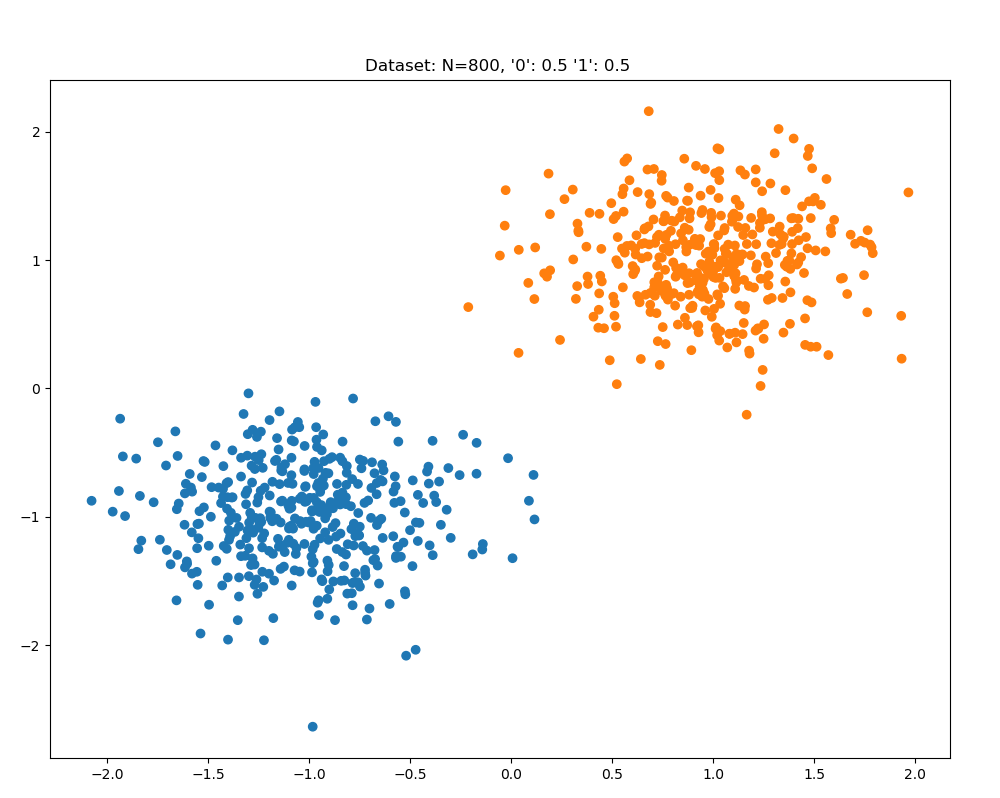
\includegraphics[width=.8\textwidth]{svm_linear_scatter.png}
        \mycaption{Linearly Seperable Data}{An artificially created dataset that is easily linearly separable}
        \label{fig:svm_lineardata}
    \end{subfigure}%
    \begin{subfigure}{.5\textwidth}
        \centering
        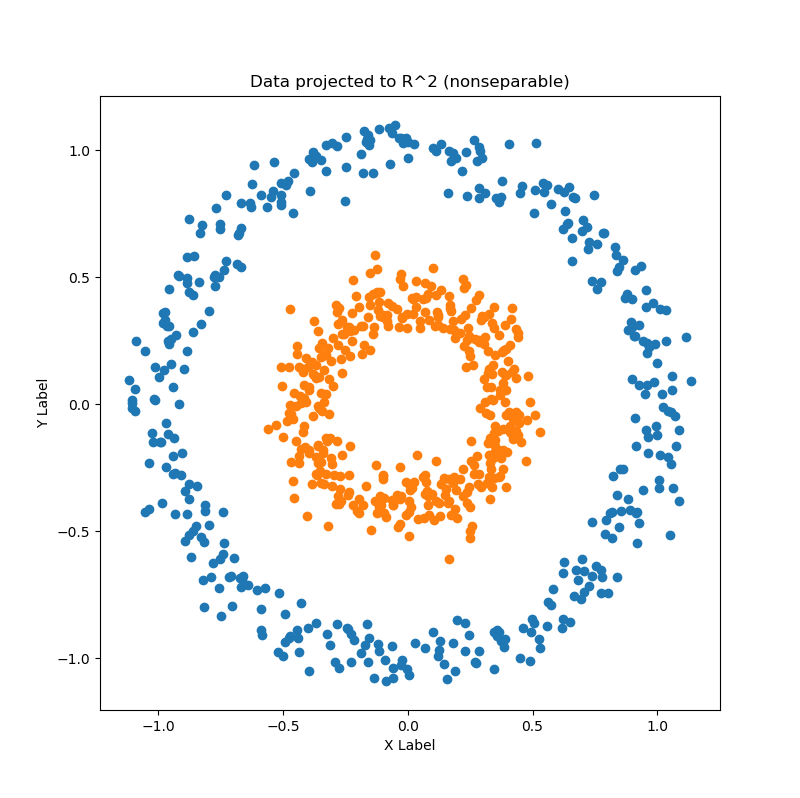
\includegraphics[width=.8\textwidth]{svm_circle_scatter.png}
        \mycaption{Non-Linearly Separable Data}{The circular data structure makes it linearly inseparable. A non linear classifier would be needed.}
        \label{fig:svm_nonlineardata}
    \end{subfigure}
    \mycaption{Example Datasets}{Artificial example datasets to illustrate the difference between linearly and non-linearly separable data.}
\end{figure}
The projection into higher space and then back again, can be expressed as the inner (dot) product of the transformation of two vectors ($\langle\phi(x_n),\phi(x_n')\rangle$) and according to Mercer's Theorem this mapping can be done independently from the explicit transformation \cite{Jordan.2004}. This computation of the inner product of the transformation of two input vectors is called a kernel. Thus a kernel $K(x,x') = \langle\phi(x_n),\phi(x_n')\rangle$ maps $K: \mathbb{R}^n\times\mathbb{R}^n\rightarrow\mathbb{R}$ the dot product of two n-dimensional vectors to a real valued scalar. Avoiding to explicitly state the transform function in this way is called the "Kernel Trick"\cite{Theodoridis.2008}. There are several kernel functions that fulfill those properties and are widely used. Most simple is the linear kernel, which is also what the examples here illustrate. In training, several kernels were tested on the dataset:
\[
\begin{array}{ll}
    \text{linear} & (\langle x,x'\rangle)\\\nonumber
    \text{sigmoidian / hyperbolic tangent} & (\tanh{(\gamma\langle x,x'\rangle+r)})\\\nonumber
    \text{polynomial} & ((\gamma\langle x,x'\rangle+r)^d)\\\nonumber
    \text{gaussian radial basis function (rbf)} & (\exp{(-\gamma\lVert x,x'\rVert^2)})\\\nonumber
\end{array}
\]
While harder to solve, non-linear kernels do perform better on smaller feature spaces than a linear kernel.
\begin{figure}[ht] % composite of 3d transform
    \centering
    \begin{subfigure}{.33\textwidth}
        \centering
        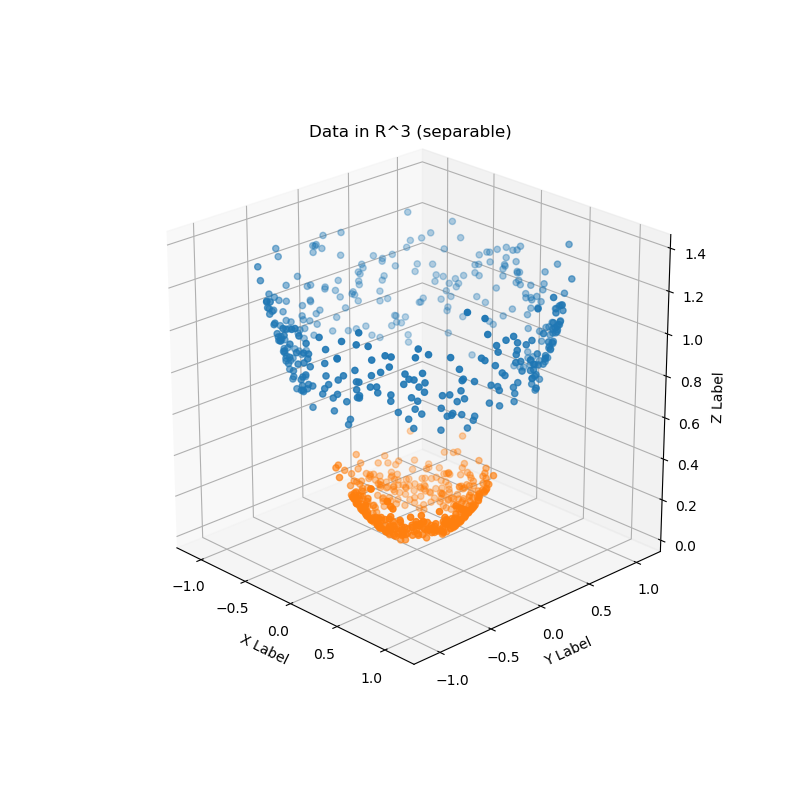
\includegraphics[width=.8\linewidth]{svm_circle_3d.png}
        \caption{}
        % \caption{The circular dataset from \ref{fig:svm_nonlineardata} projected to 3-dimensional space using $T(x,y) \rightarrow (x, y, x^2+y^2)$. The data is now linearly seperable.}
        \label{fig:svm_nonlineardata_3dprojection} 
    \end{subfigure}%
    \begin{subfigure}{.33\textwidth}
        \centering
        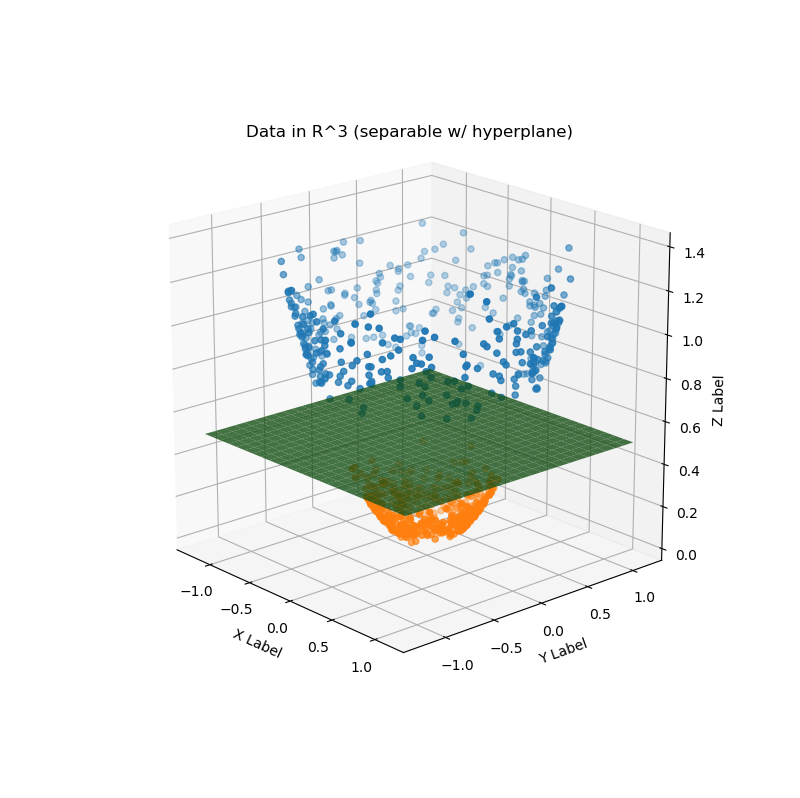
\includegraphics[width=.8\linewidth]{svm_circle_3d_hyperplane.png}
        \caption{}
        % \caption{Projected dataset with separation hyperplane.}
        \label{fig:svm_nonlineardata_3dprojection_hyperplane}
    \end{subfigure}%
    \begin{subfigure}{.33\textwidth}
        \centering
        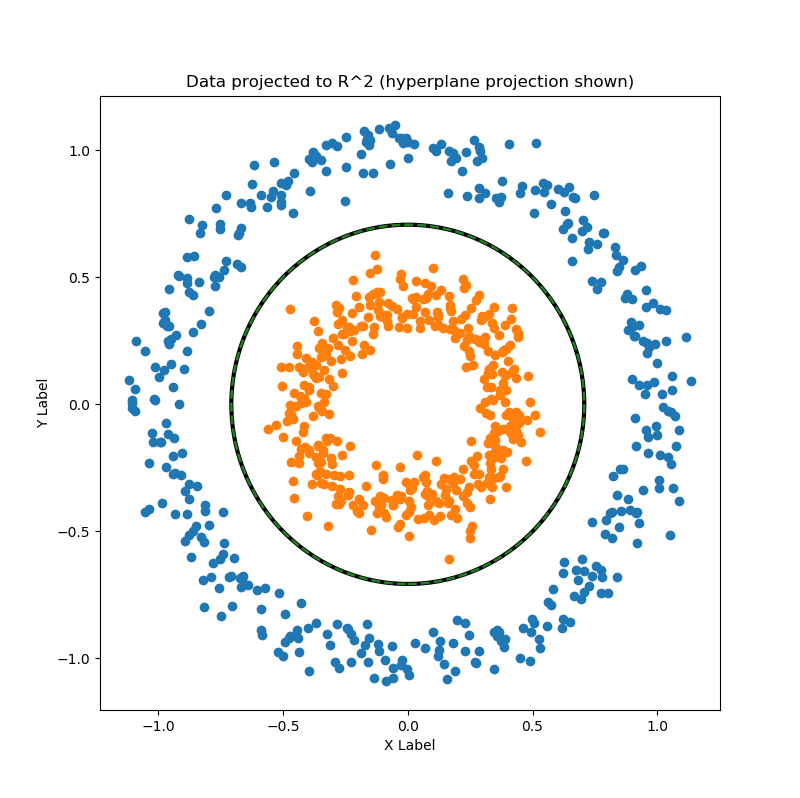
\includegraphics[width=.8\linewidth]{svm_circle_scatter_hyperplane.png}
        \caption{}
        % \caption{Data projected back into 2-dimensional space, including hyperplane projection. The linear hyperplane becomes a non-linear separation in lower dimensional space.}
        \label{fig:svm_nonlineardata_hyperplane}
    \end{subfigure} 
    \mycaption{SVM Projection Into a Higher Space}{(a) shows a possible transformation of the dataset from \ref{fig:svm_nonlineardata} to 3d space using $T(x,y) \rightarrow (x, y, x^2+y^2)$. (b) then shows a separating hyperplane that could be constructed by a SVM. (c) is the representation in 2d back from the transformed data and constructed hyperplane. The linear hyperplane now appears as a non-linear separator.
    Inspired by and derived from \cite{Kim.2013}.}
    \label{fig:svm_nonlineardata_whole}
\end{figure}

There are extensions to SVMs that allow for multiclass classification, which will not be further discussed here as they have no tangent with this work. The input vectors to SVMs must be real valued. To this day, SVMs are a benchmark for ML applications.
\FloatBarrier

\subsubsection{Decision Trees}
\FloatBarrier
Decision Trees are also known from outside computer science. The concept for decision making is the same as it is on a flowchart and as it is seen and used in offices for decision making and project management. The computer science tree and paper flowcharts function the same way. They consist of nodes and branches connecting them. The start node is called the root and if a node is terminal -- it does not branch further, it is called a leaf. Each node represents a feature, the branches from a node are the corresponding feature values and the leaves are target values. When classifying a sample, one starts at the root and then uses the feature value of the current feature node to decide which branch to follow until one reaches a leaf node. The leaf then determines the classification outcome. Decision Trees have intelligible feature weights, meaning that one can read out which features are closer to the root. The closer a feature is to the root, the higher is the importance of the information they are carrying for classification. See figure \ref{fig:dtc} for a simple example of a decision tree. Here the target variable is a binary decision of whether to go play tennis. There are three features: Outlook, wind and humidity. Where outlook has three possible values and wind and humidity have two. As such outlook has three branches to follow.\\
When building a decision tree classifier (DTC), there are several algorithms available; probably most common is the ID-3/4/5 algorithm. At each step the variable is chosen that best splits the items. What "best" means is determined by the amount of information gained by splitting. Most commonly either the gini Impurity or the information gain is used. Information gain is based on entropy and information theory and aims to maximize entropy in each selection step. Gini impurity is a measure of how often an incorrect label would be assigned, if a label would be chosen at random. Thus the gini impurity is higher for variables with less labels. ID-3/4/5 typically use the information gain and the CART (classification and regression tree) algorithm usually uses the gini impurity.\\
Decision Trees can handle categorical and numerical data, which often voids the need of encoding the data beforehand. Encoding can have unwanted side effects depending on the encoding, e.g. in onehot encoding the relation between variable values is lost. Decision trees are independent of normalization of the input data. The decision making is understandable and analogue to human reasoning and they scale well to large datasets and feature spaces. They are also able to handle multi-class problems without modification. However, they also tend to not generalize well, building overly complex trees, and tend to be unstable. Even when created from the same underlying data, the trees can vary greatly depending on which data is shown during training. With an unbalanced dataset -- some classes having more samples than others, decision trees also tend to bias towards the overrepresented class.\\
\begin{wrapfigure}{R}{6cm}
    \centering
    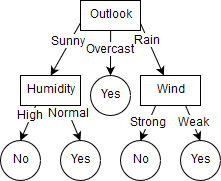
\includegraphics[width=5.5cm]{DTC_example.png}
    \mycaption{Simple DTC example}{
    A simple DTC for whether one should play tennis.
        Taken from \href{http://jmvidal.cse.sc.edu/talks/decisiontrees/allslides.htmlg}{José M. Vidal}
    }
    \label{fig:dtc}
\end{wrapfigure}
\FloatBarrier

\subsubsection{Random Forests}
\label{sec:rfc}
Random forests are an extension of decision tress. The name was coined by Tin Kam Ho \cite{Ho.1995}\cite{Ho.1998} and Leo Breiman \cite{Breiman.2001}. In a random forest classifier (RFC), several decision trees are randomly trained. There are different randomizing and training strategies. Ho suggested using random subspace sampling, meaning each tree will get a randomized subset of the input features to classify. Breiman adapted and extended it with his "bagging" approach, which creates randomized subsets with replacement, which further stabilizes the sampling and training. In order to classify an input sample, all trees are evaluated and the majority classification wins. They have the positive attributes of decision trees, namely interpretable feature weights, working on categorical data and being well scalable to large feature spaces. They also mitigate the overfitting of single trees and increase robustness. Since each tree in a forest is evaluated on its own and trained on its own, random forests are easily parallelized, which enables comparably quick training and evaluation times.

\subsubsection{Feed Forward Networks}
\FloatBarrier
Feed forward networks (FFN) belong to a subgroup of machine learning called "neural networks" or "deep learning". The feed forward network is also known as "fully connected" or "multilayer perceptron". The idea of the perceptron was proposed in 1958 to emulate the biological neuron. It was using a step function to emulate the "all-or-nothing" principle of a neuron. If the input to the perceptron was high enough, it would "fire" (output a 1, see figure \ref{fig:perceptron}). Since then the perceptron model was extended and refined. The multilayer perceptron (or FFN) is, as the name implies, several perceptrons lined up in layers. The input is fed into an array of perceptrons. The output of those is then fed into a next array of perceptrons, where each perceptron of the following layer receives all outputs of the previous layer as inputs (see figure \ref{fig:multilayer_perceptron}). The name "feed forwar network" derives from the flow of information. The data is fed from one layer in the network into the next in each step until it reaches the output. The last layer is called the readout layer. The layers in between the input and readout layer are called hidden layers. The width and depth (number of layers) can be chosen freely and optimized for the problem at hand. However, the wider and deeper a network is, the harder it is to train and the more training data is necessary, since more weights mean increased complexity. The neurons may have different activation functions than the step function. Popular choices include a sigmoidian activation, mapping the input onto the interval (0, 1), relu, which maps the input linearly if it is positive or tanh, which maps the input onto the interval (-1, 1). Depending on the task at hand, an activation function may be more or less effective. 
In a binary classification task, as it is presented in this thesis, a single neuron is enough for the readout layer. With a step or sigmoidian activation function it maps its input onto between 0 or 1, which each represents one of the target classes.
\begin{figure}[ht]
    \centering
    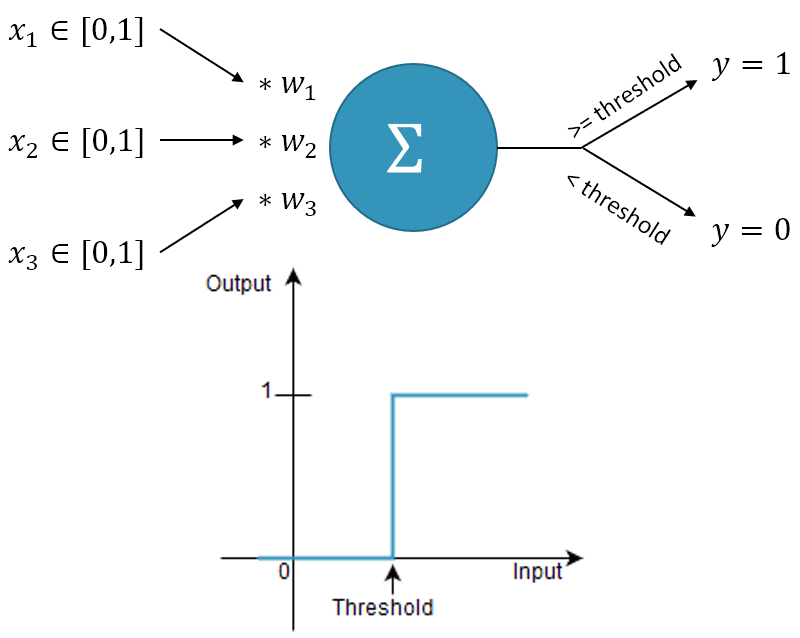
\includegraphics[width=.4\textwidth]{perceptron}
    \mycaption{A Perceptron}{A perceptron can has indefinitely many inputs. Each input is weighted and summed up. If the sum exceeds a certain threshold the perceptron "fires"}
    \label{fig:perceptron}
\end{figure}
\begin{figure}[ht]
    \centering
    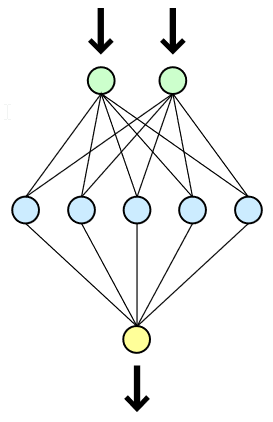
\includegraphics[width=.3\textwidth, height=.275\textheight]{multilayer_perceptron}
    \mycaption{A simple FFN}{A FFN (or multilayer perceptron) consists of several layers of neurons. Each neuron of receives all output of the previous layer as input. Each neuron has its own set of weights. The last layer is called readout, and puts out the prediction of the network.}
    \label{fig:multilayer_perceptron}
\end{figure}

\FloatBarrier
\subsection{Surveying \& Preprocessing the Data}
\FloatBarrier
\label{sec:preprocessing}
\subsubsection{Surveying}
\begin{table}[ht]
    \centering
    \mycaption{Variable Overview}{An overview of the most relevant variables for this work}
    \label{tab:dataset_variables}
    \rowcolors{2}{}{light-gray}
    \begin{tabular}{p{.13\linewidth} p{.25\linewidth} p{.52\linewidth}}
        \textbf{Variable} & \textbf{Name \& Location} & \textbf{Description}\\
        \hline
        ID\_t & All & The unique, pseudonomized id identifying a particular student\\
        spell & All spell files & The spell id for a particulat student in a particular file \\
        subspell & All spell files & Identifier whether the spell is completed and integrated or ongoing\\
        wave & CATI / CAWI & The wave the interview was in \\
        ts15218 & VocTrain%, Successful completion of vocational training program
            & The target variable holding whether the spell was completed successfully\\
        ts15201 & VocTrain & The kind of educational institution (university, university of applied science, private college, etc.)\\
        ts15221\_v1 & VocTrain & The pursued degree\\
        tg02001 & CATI & Degree of the study programme as of first interview
    \end{tabular}
\end{table}
\begin{table}[ht]
    \centering
    \mycaption{Files of NEPS used}{An overview over the used files of the dataset. Files dropped due to not providing enough data are not listed.}
    \label{tab:dataset_files}
    \rowcolors{2}{}{light-gray}
    \begin{tabular}{p{.2\linewidth} p{.525\linewidth} p{.175\linewidth}}
        \textbf{Filename} & \textbf{Description} & \textbf{\# Variables}\\
        \hline
        pTargetCATI & Computer Assisted Telephone Interview, one of two sources of information & 911\\
        pTargetCAWI & Computer Assisted Web Interview, one of two sources of information & 1285\\
        spEmp & Spells of employment & 168\\
        spGap & Gap years / spells & 27\\
        spInternship & Mandatory and voluntary internships done & 47\\
        spMilitary & Miliatrian and civilian spells & 26\\
        spPartner & Partners and relationships & 141\\
        spSchool & Primary and secondary education & 81\\
        spSibling & Siblings & 11\\
        spUnemp & Spells of unemployment & 34\\
        spVocTrain & Tertiary education and apprenticeships & 195
    \end{tabular}
\end{table}
For an overview of the variables mentioned here and the files used in preprocessing, see tables \ref{tab:dataset_variables} and \ref{tab:dataset_files} respectively.\\
In order to apply these algorithms to the NEPS dataset, the first step was to find those variables that encoded the target to predict and those that encode the data we needed to filter on. All of this information was stored in the files \textit{VocTrain} and \textit{CATI}, which hold the general information on each vocational training episode and the data of the yearly telephone interviews respectively. This information is also (partially) available in the already aggregated files. However, the general aim of this work was to introduce as little human bias as possible, while not removing the expert knowledge of a human examining a database with contextual knowledge. There seemed to be no new contextual knowledge or information inserted into the aggregated files. Hence, preaggregated files were discarded altogether. All analysis was done on the raw data, which holds equal or more information than the preaggregated files.
The variable \textit{ts15218} represented the "Successful completion of vocational training program". It is a binary variable encoding 1 for a successfully completed episode and 2 for an unsuccessful episode. Additionally there are several reasons the value may be missing (e.g. an ongoing spell, refusal to answer). The reasons for an unsuccessful episode in tertiary education were
\begin{enumerate*}[label=\alph*)]
    \item a main subject changes over the course of studies
    \item the attainable degree changes over the course of studies (e.g. from MA to teaching cert.)
    \item the education is discontinued
\end{enumerate*}.
For this work we dropped all spells in the database that are marked as ongoing spells. The status of a spell is encoded in the variable \textit{subspell}. A completed and integrated spell will have a subspell value of 0. All those spells which had missing values in ts15218 were dropped as well.

\subsubsection{Preprocessing: Cleaning and Filtering}
The overall goal of preprocessing is to create a dataframe where there is only one row for each ID\_t-spell pair of interest.\\
Since the analysis was only aimed at bachelor students, all spells that corresponded to master students, apprenticeships, PhDs, etc. needed to be dropped as well. In VocTrain the variable \textit{ts15201} encoded what kind of educational institution the student was located at. Only rows were kept which had a value of 10 for a university, 9 for a university of applied science or -28, which meant that this information was to be found in CATI variable \textit{tg02001} and was part of the initial questionnaire. Next we only kept students which were actually studying in a bachelor program. This information was for one encoded in tg02001 in CATI with the values 1 and 3 for bachelor of education and all other bachelor programs respectively, and second in \textit{ts15221\_v1} which encoded 8, 12, 13 for "general bachelor program", "bachelor of education" and "bachelor", excluding bachelor of education. Why the distinction between 8 and 13 was made remained unclear. There were three versions of \textit{ts15221}: the original one, version 1 and generated 1. The decision to use version 1 was made, since that version had the least missing values and as such seemed to be of most use. The generated (in this case called "corrected") version held no information on any bachelor student and as such was deemed to be uninformative for this work. From this filtered version of the NEPS dataset, all combinations of \textit{ID\_t} and \textit{spell} were extracted. Those two values uniquely identify all spells of interest for this work: students that completed or dropped out of a bachelor degree program. This leaves us with a total of 9551 spells of interest out of 39642 total vocational spells in the dataset, with a split of 6454 successful and 3097 unsuccessful spells, roughly a 2:1 split, for our classes (see figure \ref{fig:classbalance}).
\begin{figure}[ht]%{L}{width=.3\textwidth}
    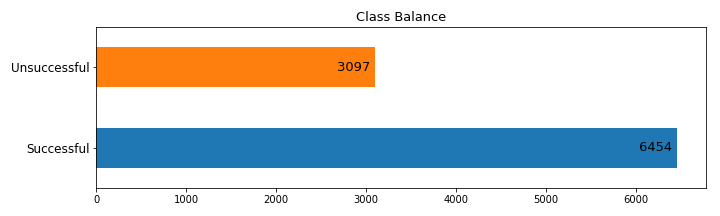
\includegraphics[width=\textwidth]{classbalance_hrz.png}
    \mycaption{Class Balance of the Dataset}{The class balance of the targets. Giving a rough 2:1 split.}
    \label{fig:classbalance}
\end{figure}
Now that the target variable is set up, and unique identifiers of educational spells of interest are available, the rest of the available data needs to be cleaned, aggregated and joined into one coherent dataframe with one row per spell. Each spell is a sample and as such should be represented by a single vector.

In order to reduce the size of the resulting dataframe, not all files were included in the aggregation. If a file contained less than 45\% of the relevant student ids, they were dropped. They would inflate the overall resulting vector without supplying a proportionate amount of information. In the end eleven files remained: Sibling (spSibling), Military (spMilitary), Gap (spGap), Unemployment (spUnemp), Internship (spInternship), School (spSchool), Partner (spPartner), Employment (spEmp), CAWI (pTargetCAWI), CATI (pTargetCATI), Vocational Training (spVocTrain).\\
A rather large part of the data was missing for different reasons. Most often it was "missing by design". Variables holding e.g. sex, date of birth or the perceived job chances for the student's phd are not meant to be asked every time. They either do not change and are hence only asked once or are not relevant to all interviewees; questions on siblings are not relevant to a single child and questions on the current phd program have no meaning when a bachelor student is asked. Sometimes there were also other reasons (e.g. questions not reached, implausible value, answered "don't know") for missing data. Values marked as "missing by design", "unspecified missing" or "does not apply" were firstly coded as NaN. The wave data of CATI and CAWI was then grouped by student id and examined in those groups. Each column which only held exactly one value in one cell and was NaN for the rest, would then have that one value copied into all the NaN cells of this variable. The underlying assumption was that a column being all NaN beside a single value were questions that were only necessary to ask once and as such the information is relevant to all waves. When cleaning the data several values were replaced as NaN instead of featuring them as a category on their own, and mostly variable specific missing values were kept (see table \ref{tab:missing_value_treatment} for an overview).\\
\begin{table} % handling of missing values
    \centering
    \mycaption{"Missing Values" Categories}{An overview of values representing a missing entry and how they were treated}
    \label{tab:missing_value_treatment}
    \rowcolors{2}{}{light-gray}
    \begin{minipage}{.5\textwidth} % recoded as NaN
        \centering
        \begin{tabular}{l| l}
            \multicolumn{2}{c}{Considered NaN}\\
            \hline
            \textbf{Value} & \textbf{Name}\\
            \hline
            -94 & not reached \\ 
            -95 & implausible value \\ 
            -98 & don't know \\ 
            -54 & missing by design \\ 
            -90 & unspecified missing \\ 
            -93 & does not apply \\ 
            -99 & filtered \\ 
            -52 & implausible value removed \\ 
            -53 & anonymized \\ 
            -55 & not determinable \\ 
            -56 & not participated     
        \end{tabular}
    \end{minipage}%
    \begin{minipage}{.5\textwidth} % contained as category
        \centering
        \begin{tabular}{l| l}
            \multicolumn{2}{c}{Considered Category}\\
            \hline
            \textbf{Value} & \textbf{Name}\\
            \hline
            -97 & refused\\
            -29 & variable specific \\
            -28 & variable specific \\
            -27 & variable specific \\
            -26 & variable specific \\
            -25 & variable specific \\
            -24 & variable specific \\
            -23 & variable specific \\
            -22 & variable specific \\
            -21 & variable specific \\
            -20 & variable specific \\
        \end{tabular}
    \end{minipage}
\end{table}
Since many of the variables are available in different versions, those needed to be reduced to a single column to remove redundancy. Variables with the suffix \textit{O} or \textit{R} were anonymized for the downloaded version and as such discarded. Variables with the suffix \textit{w} are stored in wide format and belong together. As such they were not altered. Variables that had a suffix of \textit{v} or \textit{g} indicating that this variable was altered in some way. Versioned variables (v suffix) were often corrected for implausible values or held corrected information. Generated variables (g suffix) were often reconstructed or created with a better formal fit from the underlying data. For date variables (those whose identifier ends in m or y without suffix) the generated versions were kept as a general rule, as they were corrected to fit into the 1-12 month range instead of having values like "end of summer", and correctly labeled missing values if a date was not parsable. For all other variables that had multiple versions available the one with the least NaN values was chosen as a heuristic for being the most informative version. Keep in mind that this is after a selection of missing denominations were already replaced with NaN, which should lead to the variable with the least NaN values also being the one with the most cells containing actual information (non missing values).

\subsubsection{Preprocessing: Aggregation}
The key values uniquely identifying a vocational spell of interest are ID\_t and spell. Although this applies only to VocTrain, since the spell variable is specific to one particular data file. This means that we do have only one row per sample in VocTrain already, but all other files hold several rows for each student. Those rows need to be condensed into a single row so that they can easily be appended to the rows of the corresponding student. The specific ways to condense each file needed to be written specifically for each file in such a way that all relevant information is retained. The hard question to solve then is which information in each file is indeed relevant. For the CATI and CAWI file, only the first wave was kept. Since unique information was copied to all waves, the static variables are all available in this wave. Furthermore, around 60\% of the spells of interest start in the first wave or beforehand. As such the first wave carries the most relevant information for most spells. In a more time exhaustive measure it would have been possible to identify the most recent wave for each spell and join those accordingly. However, due to resource limitations this approach was not chosen. For the spell files, the goal was to introduce as little bias as possible while not ignoring the contextual knowledge a human observer has when identifying relevant information. The information that is considered relevant was identified in a three-step process. First a human observer would get an overview of the file at hand and try to identify variables he deemed relevant and mark those. In this case, the human observer was the author. In a second step, a Random Forest Classifier with 10'000 trees(see \ref{sec:rfc}) was trained using only the file variables as features to predict the goal variable located in VocTrain, joined on ID\_t. The feature importances and their standard deviations were then extracted and analyzed. %(for plots of the feature importances see \ref{apx:methodology}).
The results were then compared with the variables chosen by the human observer. It was then determined which variables to keep, which to discard and where to aggregate several variables into a new feature. Depending on the context either the mean, mode, median or most recent value of a variable was used. The mean was always rounded to the nearest integer to reduce the amount of values per variable. However, before filtering and applying those rules, for every student in each file, all spells were removed that started after the end of the latest vocational spell of interest of that student. Information in those spells would have had little to no impact on the life and study success of students before they started. For those few students whose last vocational spell of interest ended before 2010 and thus before any other spells were recorded, only the earliest entry of each file was taken into account. This does muddy the results a little. But considering that we had less than 2\% of those students in the dataset, the advantage of having more data on those 164 seems to outweigh the disadvantages. The rules for each file were as follows:

\noindent\textbf{School:} The spSchool file provides a rather large dataset. The first four subjects of the "Abitur" are recorded as they had a relatively high feature importance. The start and end year was recorded. In other spell files the month was more relevant. Additionally the points awarded in math and german were used. Lastly, the grade of the latest school certification was taken into account, as it was by far the strongest indicator. Especially the grade was congruent with the human predictions. The kind of certificate (Abitur, Fachabitur, other) had a rather low importance and as such was not included. It was however one of the predicators humanly chosen. Though, this might have canceled out with the types of tertiary education. When predicting it was not differed between private or public universities, universities of applied science, etc.
\\
\textbf{Sibling:} For the spSibling file a new variable was created identifying the student as the youngest or oldest or being in between. Furthermore, the mode of the highest leaving certificates of the siblings was used as well as how many different leaving certificates the siblings had. This was, because the highest obtained degree of siblings was a strong indicator for academic success. The second variable was compiled as a measure of the variance in education. The predicators for siblings were rather congruent with the human predictions. The relative age of the student compared to his siblings was taken from the human made predictions; the classifier ranked the birth month and year of the sibling as the highest predicator for study success of the student.
\\
\textbf{Gap:} For all variables in the spGap file the median was used. The type of gap year was taken into account (vacation, side job, internship, etc. as well as start and end month of the episode. Again this was rather congruent with the human predictions. However, there exists a variable for "training programs during gap" which looked promising but showed little importance in the classifier result and as such was excluded.
\\
\textbf{Military:} For all variables in the spMilitary file the median was used. The type of military episode (military service, civilian service, etc.) whether seminars were attended during that episode and the start and end month were used for further processing. Here the classifier confirmed the main variables humanly predicted: the type of military episode and whether trainings were attended during that period.
\\
\textbf{Unemployment:} Start and end month in the spUnemp file were recorded as median. Furthermore, the mean number of applications send out in that period as well as the mean number of interviews the student underwent. Most of the variables identified by the human observer were not of high importance in the classifier. However, all features with high importance were also selected by the human observer. Variables about whether the student received unemployment benefits and whether she participated in programs for further education by the employment agency were cut from the set.
\\
\textbf{Internship:} In the spInternship file the median of start and end month were recorded. Furthermore, the mean of the average working time and the mean remuneration of all jobs was used. The only variable from the human set that was dropped was the one indicating what kind of internship it was (obligatory, part of a course, voluntary).
\\
\textbf{Partner:} Start and end month are recorded in spPartner, as well as the mean average working hours and the mean contact frequency. Interestingly, variables about cohabitation, marriage and vocational qualification of the partner, which were all selected by the human observer, had little relevance in the classifier. The included variables were in the set of the human observer as well as having a high feature importance.
\\
\textbf{Employment:} For the spEmployment file other factors than start and end month were more relevant. Which lined up better with the human made predictions. The median of "relation to studies" was used. The mode of the job categories and required education was assessed. Lastly the mean of the weekly working hours, gross income and net income were used. The only variables selected by the human observer that were left out, were the job category and the professional position (employee, freelancer, civil servant, etc.).

The start and end month of nearly all spell files had a high importance for the prediction of study success. The derived assumption was that a start or end too close to the semester border dates would imply a more stressful start or missing out in the exam phase. Plotting the start and end months of each file however were hardly indicative (Figure \ref{fig:spell_start_end_months}). Generally ther were more starts in the summer and more ends in the winter. The winter semester might be the more heavily impacted. However, it is not visible whether these spells actually took place during the studies or after or before. As such, there seems to be no clear indication that it falls into highly relevant parts of the semesters.
\begin{figure}
    \centering
    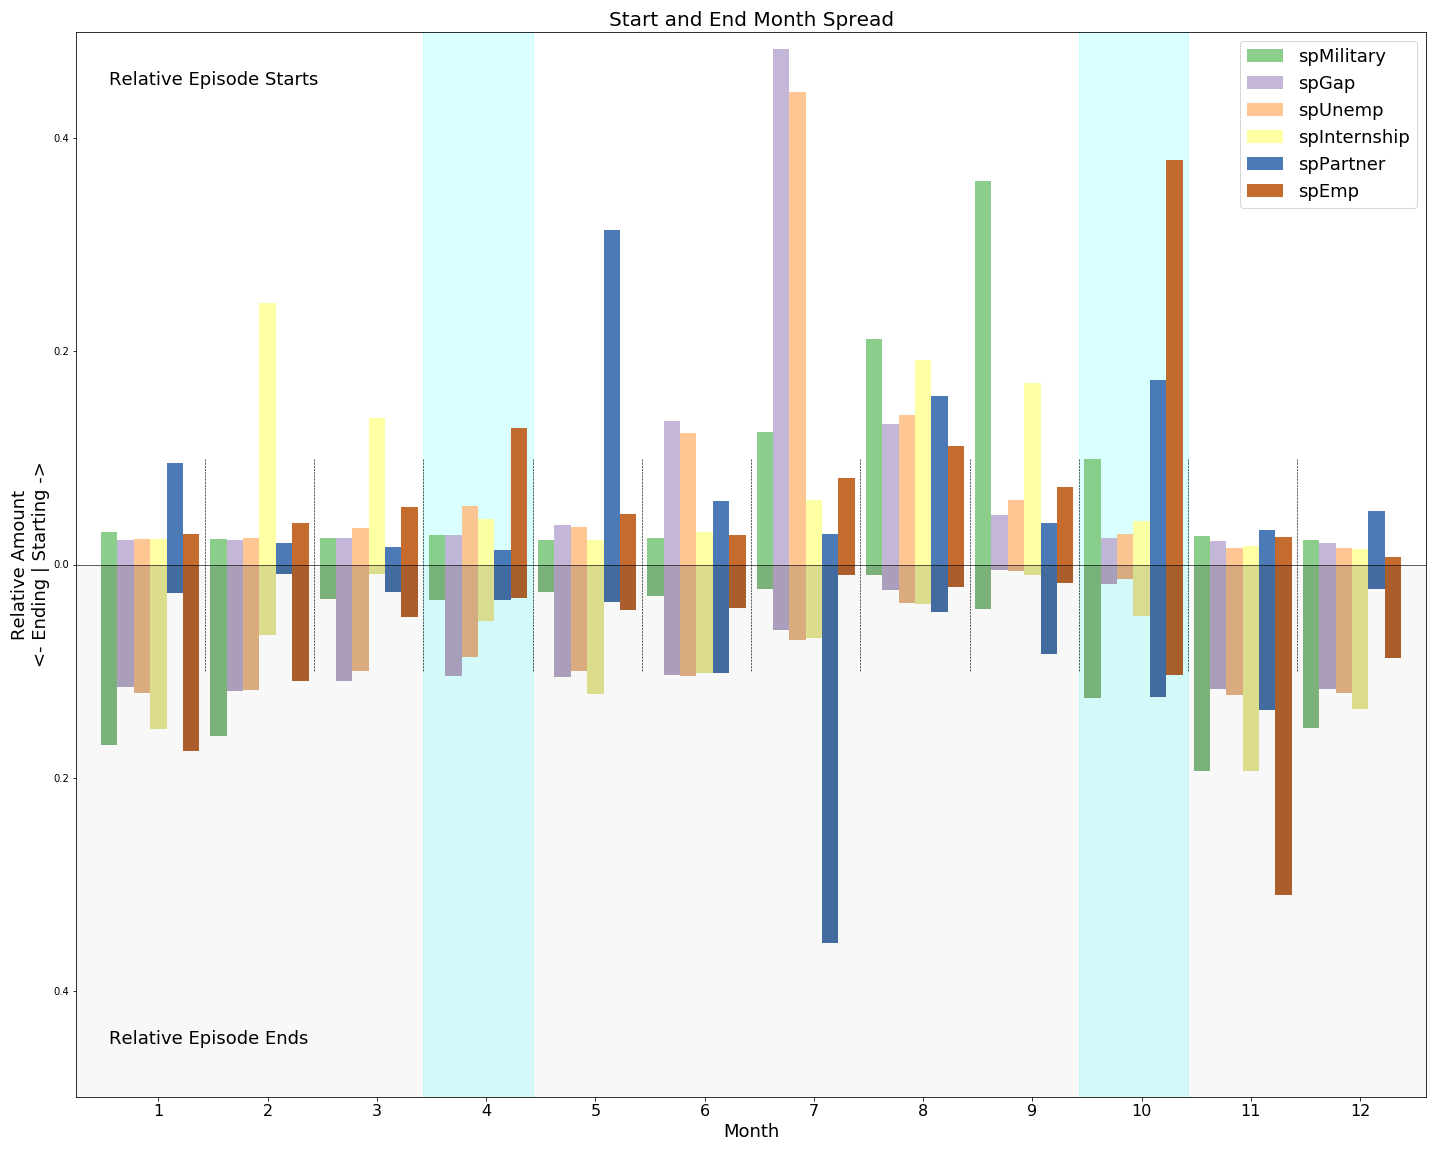
\includegraphics[width=\textwidth]{spell_start_end_months.png}
    \mycaption{Spell Start and End Months}{The relative distribution of start months -- brightly colored, top half -- and end months -- darker colored, bottom half -- of each file are plotted. The cyan bars mark the start of the summer and winter term respectively (April and October). The data was normalized per file per column. Meaning the start months of each file add up to 1 and so do the end months.}
    \label{fig:spell_start_end_months}
\end{figure}

Finally, for every student only one row per file persists and the data can be joined into one coherent dataframe. In this procedure the base for the dataframe was the VocTrain file. Only the spells of interest were selected by performing an inner merge of the VocTrain file with the data frame of unique keys (ID\_t-spell combinations). Afterwards all aggregated dataframes were subsequently joined. The final dataframe was then cleaned by dropping all columns that were more than 75\% NaN. If a variable only held information on 25\% of the students in the spells of interest, it will be hard to generalize for this variable. Hence, those variables were dropped. Furthermore, all NaN values remaining in the dataframe were replaced with $-1$, since the ML algorithms cannot handle NaN data. Finally some columns that only held organizational information were dropped from the dataset like ID\_t, variables starting with tx, as those are the identifier for the survey instrument, the spell identifier as well as subspell and spelldisalignment variables, wave information and version information.\\
The final dataframe than had the shape of $9551 \times 885$, nearly 11 times as many samples as features to learn.

\FloatBarrier
\subsection{Training}
\label{sec:training}
Grid-Parameter-Search was used for the training process and hyperparameter optimization of the random forest classifier, decision tree classifier and support vector machine classifier, using k-fold cross validation with 5 folds. The gridsearch algorithm takes a list of values for parameters (e.g. a list of kernels, a list of gamma values and a list of error coefficients for the SVM), and then exhaustively uses all possible parameter configurations possible. The amount of different configurations tried in grid searching can be calculated by $\Pi_{i}^N length(parameter_i)$, where N is the number of parameters supplied to the grid search, i is identifying one particular parameter and $length$ is the amount of possible values passed for this parameter. Performance evaluation was measured in four tests: precision, recall, f1 and balanced accuracy. They all are building on the concepts of true and false positives and negatives. A true positive is a correctly identified target, whereas a false positive is an input labeled as true, even though it was a negative sample. For the case considered in this thesis, "positive" and "targets" are unsuccessful study spells.\\
Precision is the fraction of true positives positives out of all inputs labeled as positive. It is calculated by $\frac{TP}{TP+FP}$, where $TP$ are true positives and $FP$ are false positives. Optimizing for precision means to lessen the number of false positives, while the number of false negatives is irrelevant. Thereby minimizing the amount of samples incorrectly labeled as positive, but not necessarily maximizing the amount of correctly labeled positives samples.\\
Recall is the fraction of true positives out of all samples identified as positives (which includes true positives and false negatives). It is calculated by $\frac{TP}{TP+FN}$, where $FN$ are false negatives. Optimizing for recall means to maximize the amount of correctly identified positive samples with a disregard for false positives.\\
f1 is a combined score of recall and precision calculated by $2*\frac{precision * recall}{precision + recall}$. It is the harmonic mean of the two scores. While this does build a unified score, it also ignores true negatives completely which may lead to worse overall results\cite{Powers.2011}.\\
Balanced accuracy is an accuracy measure that is corrected for imbalanced datasets. Accuracy is defined by $\frac{TP+TN}{TP+TN+FP+FN}$, where $TN$ are true negatives. Balanced accuracy on the other hand, is the average of all recalls: $\frac{\sum_{i=0}^{N}recall_i}{N}$, where $N$ is the amount of classes in the dataset and $recall_i$ identifies the recall of the i-th class.\\
Due to implementation one score had to be specified to identify the best model of the grid search. For this, recall was chosen, since optimizing for recall should lead to an increase of true positives and a decrease of false negatives. This should maximize the identification of unsuccessful study spells. Although it may also lead to an increase of false positives. Wrongly labeling students as likely to fail in their studies might have negative consequences on them, depending on the context such predictions are made and used (see \ref{sec:discussion}). Optimizing for a single score is not the optimal approach, since good performance in one test, does not necessarily indicate good performance in all other tests. A manual evaluation was necessary in the end and the optimal grid candidate according to the grid-search algorithm was not used (see \ref{sec:results}).\\
For the training process of the feed-forward network, the stage of automatic hyperparameter optimization was not reached. Already in the manual phase of testing several hyperparameter configurations, it was clear that no sufficient performance is going to be achieved. Some combinations of parameters, especially very wide networks, were not testable due to computational limitations.

Since the data seems to have no information on the variables' measurement scale, all variables were handled as being nominal. The main file format of the supplied data, does not store measurement scales, and while the alternative supplied file format does have that information, it was incorrect. IDs of students and institutions (an ever increasing integer) was labeled as interval scale and Likert scales marked as nominal. Due to time limitations, labeling all remaining 885 variables by hand was unfeasible. Since SVMs and FFNs cannot handle nominal data, the whole dataset needed to be onehot encoded. Onehot encoding, also called dummy encoding, transforms a variable into a multi-dimensional variable space, with as many dimensions as the variable has unique values. This decouples the variable values. For example, a variable for sex might have the values "male", "female", "other", represented by the values 0, 1, 2. If these values are interpreted as a real valued variable, 1.5 would need to be meaningful and "female" would be half of "other", but double of "male". When this variable is onehot encoded, the values will be represented as a three dimensional vectors: (1, 0, 0), (0, 1, 0), (0, 0, 1). Each of these dimensions represents one of the former values. All three values can now be represented independently of  each other.\\
After onehot encoding, the dataset was blown up to a size of $9551 \times 14391$, giving a mere 0.66 factor of samples to features. The onehot encoded data also provides less information as relations between ordinal and interval variable values are lost as well. The DTC and RFC were then trained on the original dataset, and the SVM and FFN on the onehot encoded dataset.\\
All classifiers were trained with the "class\_weight" set to "balanced". This automatically impairs a higher training weight on underrepresented classes, so that errors on those predictions have a higher impact. RFC had some additional constant parameters, that did not change over the grid search. All RFC were trained with 8000 estimators and bootstrapping enabled, meaning that features are randomly sampled with replacement. For the SVM only valid parameter configurations were sampled (e.g. the degree variable was not used when training the linear kernel). $C$ is the coefficient of the error term when training the SVM. For an overview of the parameters values used in the grid search see table \ref{tab:grid_search_params}.
\begin{table}
    \centering
    \mycaption{Gridsearch Paramter Grid}{An overview of the parameters supplied to the grid search algorithm}
    \label{tab:grid_search_params}
    \begin{tabular}{p{.1\textwidth} | p{.1\textwidth}p{.1\textwidth}p{.1\textwidth}p{.1\textwidth}p{.1\textwidth}}
        \textbf{Model} & \multicolumn{5}{c}{\textbf{Parameters}}\\
        \hline
                                & Kernel        & $C$     & $r$ & $\gamma$  & $d$\\
        \hline    
        \multirow{4}{*}{SVM}    & Linear        & 1     & 0     & scaled    & 3\\
                                & Polynom       & 10    & 1     & 0.001     & 5\\
                                & Sigmoid       & 100   &       & 0.0001    & 7\\
                                & rbf           &       &       & 0.00001   &\\
        \hline
                & \multicolumn{2}{l}{Min Samples per Leaf} & \multicolumn{2}{l}{Min Samples per Split} \\
        \hline
        \multirow{3}{*}{DTC}    & \multicolumn{2}{l}{1} & \multicolumn{2}{l}{2} \\
                                & \multicolumn{2}{l}{2} & \multicolumn{2}{l}{3} \\
                                & \multicolumn{2}{l}{5} & \multicolumn{2}{l}{5} \\
        \hline
                & \multicolumn{2}{l}{Min Samples per Leaf} & \multicolumn{2}{l}{Min Samples per Split}\\
        \hline
        \multirow{3}{*}{RFC}    & \multicolumn{2}{l}{1} & \multicolumn{2}{l}{2} \\
                                & \multicolumn{2}{l}{2} & \multicolumn{2}{l}{3}\\
                                & \multicolumn{2}{l}{5} & \multicolumn{2}{l}{5}\\
    \end{tabular}
\end{table}